% Please use LuaLaTeX or XeLaTeX for compilation
%\documentclass[11pt,aspectratio=169]{beamer}
\documentclass[11pt,aspectratio=169,handout]{beamer} % faster compilation without animation

% Theme and Colors
\usetheme{eth}
\colorlet{titlefgcolor}{ETHBlue}
%\colorlet{titlefgcolor}{ETHGray}
\colorlet{accentcolor}{ETHBlue}
%\colorlet{titlebgcolor}{ETHPetrol} % Title slide background

% Standard Packages
\usepackage{amsmath,amssymb,amsthm,mathtools,mathrsfs,braket} % Math symbols
\usepackage{bm} % Bold math symbols
\usepackage{graphicx} % Include graphics (if needed)
\usepackage{booktabs} % Nicer tables (if needed)
\usepackage{microtype} % Better typography

% Ben packages
\usepackage{soul}
\usepackage{multimedia}
\usepackage{media9}

% Chung-En
\setbeamercolor{frametitle}{fg=ETHBlue} % set color of frame title
\usefonttheme{professionalfonts}
\usepackage{eulervm}
\DeclareMathOperator{\E}{E}
\DeclareMathOperator*{\argmax}{arg\,max}
\DeclareMathOperator*{\argmin}{arg\,min}
\useinnertheme[rounded,shaded=false]{tcolorbox}
\setbeamercolor{block body}{fg=black,bg=white}
\makeatletter
\tcbset{
  	boxrule=1pt,
  	borderline={1pt}{0pt}{beamer@tcb@titlebg},
}
\makeatother

% footnote for reference (added by Chung-En)
\definecolor{DarkGray}{RGB}{124,124,124}
\newcommand\reffootnote[1]{%
\begingroup
\renewcommand\thefootnote{}\footnote{\hspace{-20px}\color{DarkGray}#1\vspace{5px}}%
\addtocounter{footnote}{-1}%
\endgroup
}

% Citation Management (using biblatex)
\usepackage[style=numeric, backend=biber]{biblatex}
\addbibresource{references.bib} % You need a references.bib file

% Footnotes (optional, if needed)
\usepackage[multiple]{footmisc}
\usepackage{footnoterange}
\usepackage{fnpct}
\AdaptNote\footcite{oo+m}[footnote]{%
\setfnpct{dont-mess-around}%
\IfNoValueTF{#1}
{#NOTE{#3}}
{\IfNoValueTF{#2}{#NOTE[#1]{#3}}{#NOTE[#1][#2]{#3}}}%
}

% Algorithms (optional, if needed)
\usepackage{algorithm}
\usepackage[noend]{algpseudocode} % Use noend option as in template

% Tikz/PGFPlots (optional, if needed for diagrams)
\usepackage{tikz}
\usetikzlibrary{shapes, arrows, positioning, calc}
\usepackage{pgfplots}
\pgfplotsset{compat=1.17} % Use a recent compatibility level

% Custom command for highlighting math
\newcommand\mathalert[1]{{\color{accentcolor}#1}}



% --- Presentation Metadata ---
\title{Paper Presentation: ``Optimistic Active Exploration of Dynamical Systems''\vspace{0.1in}\\
\small Based on the work of Sukhija et al. (NeurIPS 2023)}
\subtitle{Based on Sukhija et al. (NeurIPS 2023)} % Use subtitle for source
\author{Chung-En Tsai \and Ben Bullinger} % Presenters
\institute{ETH Zürich \\ Department of Computer Science}
\date[FoRL Spring 2025]{Foundations of Reinforcement Learning (263-5255-00L), Spring 2025} % Course info and date

\begin{document}

% --- Title Slide ---
\def\titlefigure{elements/title-page-image}  % No figure on title slide unless specified
\setlength{\titleboxwidth}{0.85\textwidth} % Adjust box width if needed
\titleframe % Creates the title slide using the theme's definition

% --- Table of Contents ---
\tocframe % Creates the table of contents slide

% --- Section 1: Introduction ---
\section{Introduction}

\begin{frame}{Motivation: Beyond Task-Specific Models}
    \begin{itemize}
        \item \textbf{Standard MBRL Goal:} Learn dynamics model $f$ to solve a \textit{specific} task (maximize reward $R$).
        \item \textbf{Problem:} Exploration driven by task reward $R$ leads to biased models.
        \begin{itemize}
            \item Agent only learns dynamics well in task-relevant state-action regions.
            \item Model fails to generalize to \textit{new} tasks requiring different parts of the state space.
            \end{itemize}
        \item \textbf{Need:} Methods to learn \textit{globally accurate} models, useful for \textit{any} downstream task.
        \pause
        \item \textbf{Idea:} Decouple exploration from extrinsic rewards. Explore to gain \textit{information} about the system itself.
    \end{itemize}
    \vspace{1em}
    \begin{alertblock}{Goal of Task-Agnostic Exploration}
        Interact with the environment to build a dynamics model $\hat{f}$ that is accurate everywhere, enabling \textit{zero-shot} (or few-shot) generalization to new tasks.
    \end{alertblock}
\end{frame}

\begin{frame}{Introducing OPAX}
    \begin{itemize}
        \item \textbf{OPAX:} Optimistic Active Exploration of Dynamical Systems \footcite{sukhija2023optimistic}.
        \item \textbf{Core Idea:} Frame exploration as Bayesian optimal experimental design.
        \begin{itemize}
            \item Actively seek interactions (trajectories) that maximally reduce \textit{epistemic uncertainty} about the unknown dynamics $f^*$.
        \end{itemize}
        \pause
        \item \textbf{Key Components (Overview):}
        \begin{enumerate}
            \item \textbf{Probabilistic Model:} Quantifies belief and uncertainty about $f^*$ (e.g., Gaussian Process, Ensemble).
            \item \textbf{Information Gain Objective:} Formalizes uncertainty reduction as the goal.
            \item \textbf{Optimistic Planning:} Plans trajectories assuming the "most informative" plausible dynamics.
        \end{enumerate}
    \end{itemize}
    \vspace{1em}
    \begin{block}{Promise of OPAX}
        Learn general-purpose world models efficiently, enabling robust planning and control across diverse tasks without task-specific retraining.
    \end{block}
\end{frame}

% --- Section 2: Problem Statement ---
\section{Problem Formulation}


\begin{frame}{Problem Formulation (1/2)}
% \begin{block}{Problem}
Given an \textcolor{ETHRed}{unknown} discrete-time dynamical system $f^\star:\mathcal{S}\times\mathcal{A}\to\mathcal{S}\subseteq\mathbb{R}^d$:
\[
    s_{t+1} = f^\star(s_t,a_t) + w_t, \quad w_t\sim\mathcal{N}(0, I).
\] 
Goal: Design algorithms for learning $\hat{f}\approx f^\star$ that is good for any reward functions in episodic setting:
% \begin{itemize}
%     \item We \textcolor{ETHRed}{cannot} query $f^\star$ at arbitrary state-action pair.
%     \item We \textcolor{ETHRed}{can} roll out  policies and observe trajectories.
% \end{itemize}
% \end{block}

\begin{center}
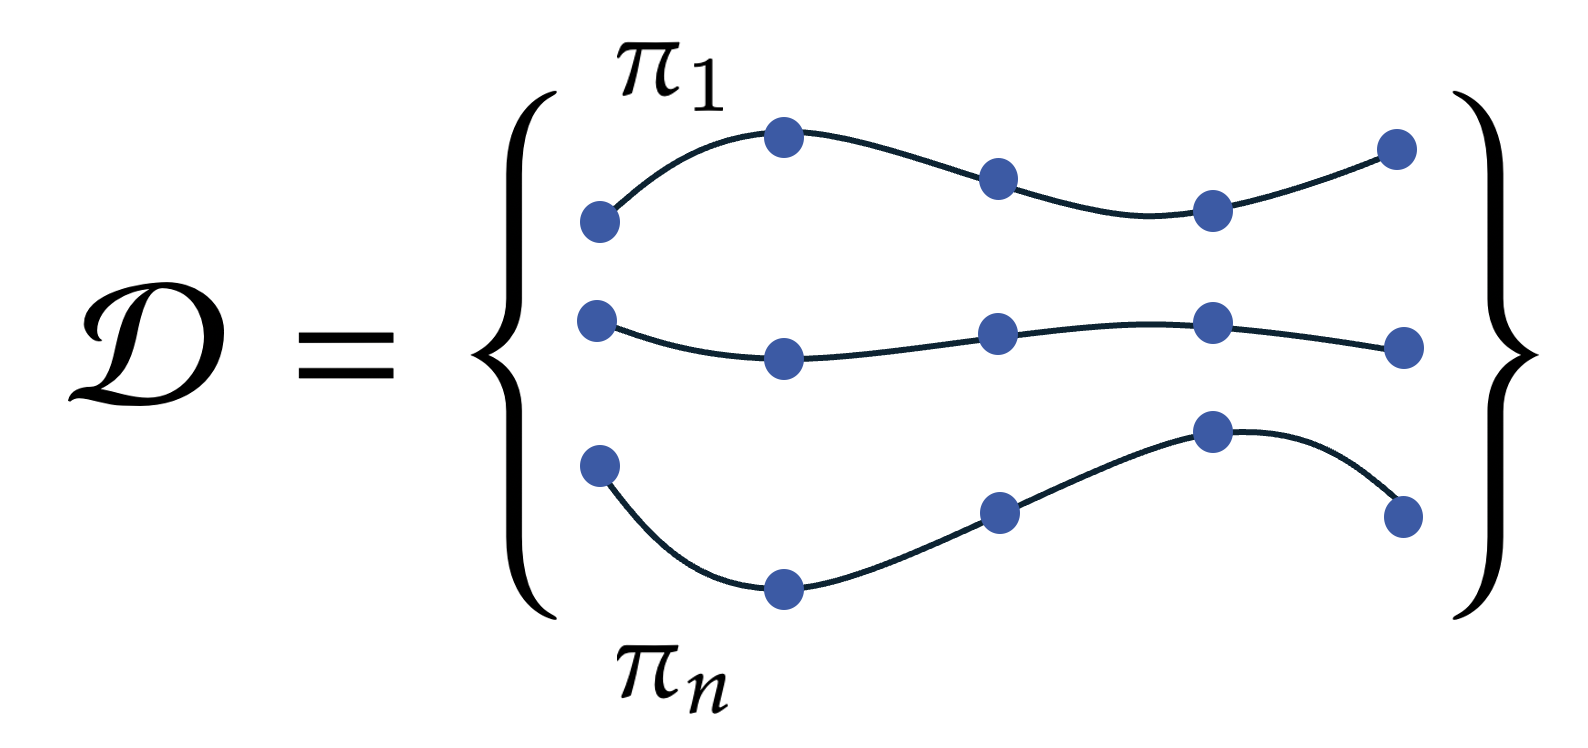
\includegraphics[scale=0.25]{Latex_Praesentation/figures/dataset.png}
\end{center}


% \begin{alertblock}{Goal}
%     Design a theoretically grounded algorithm for learning $\hat{f}\approx f^\star$ that is good for any reward functions.
% \end{alertblock}
\reffootnote{Introduction video by Bhavya Sukhija. NeurIPS 2023.}

\end{frame}


\begin{frame}{Problem Formulation (2/2)}


Our problem can be divided into two parts:
\begin{itemize}
    \item \textcolor{ETHRed}{Exploration (our focus!):} Collecting data by executing policies.
    \item Estimation: Building model from data.
\end{itemize}

\begin{block}{Well-Calibration Assumption}
    Given $n$ data, we can construct confidence intervals:
    \[
        \lvert f^\star_i(s,a) - {\color{ETHRed}\mu_{n,i}(s,a)} \rvert
            \leq {\color{ETHRed}\beta_n \sigma_{n,i}(s,a)} \quad \forall i\in[d],\ \text{w.h.p.},
    \]
    \begin{center}
    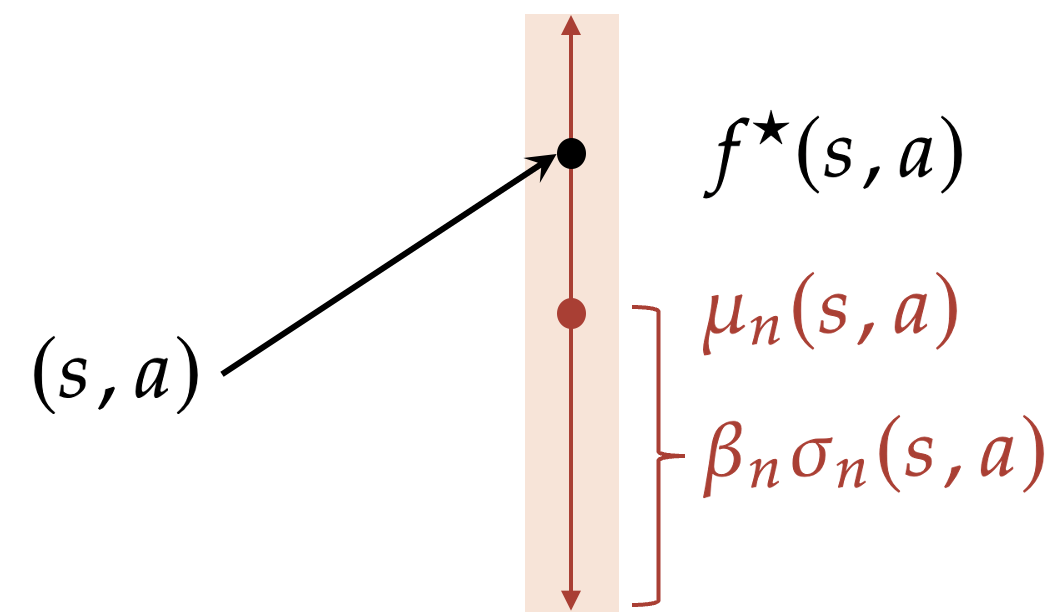
\includegraphics[scale=0.25]{Latex_Praesentation/figures/confidence_interval.png}
    \end{center}
\end{block}

\end{frame}


% \begin{frame}{Challenges}



% \end{frame}



% \begin{frame}{System Dynamics and Objective}
%     \begin{itemize}
%         \item Consider a discrete-time stochastic dynamical system:
%             \[ x_{k+1} = \mathalert{f^*(x_k, u_k)} + w_k \]
%             \begin{itemize}
%                 \item $x_k \in \mathcal{X}$: State
%                 \item $u_k \in \mathcal{U}$: Action
%                 \item $\mathalert{f^*}$: Unknown true dynamics function
%                 \item $w_k$: Noise (aleatoric uncertainty), e.g., $w_k \sim \mathcal{N}(0, \sigma^2 I)$
%             \end{itemize}
%         \pause
%         \item \textbf{Goal:} Learn a model $\hat{f}_N$ after $N$ episodes (each horizon $T$) that accurately approximates $f^*$ over the \textit{reachable state-action space} $\mathcal{R}$.
%             \[ \mathcal{R} = \{ (x, u) \mid \exists \pi, t<T \text{ s.t. } p(z_t = (x,u) \mid \pi, f^*) > 0 \} \]
%         \pause
%         \item \textbf{Measure of Success:} Reduction in \textit{epistemic uncertainty} (uncertainty about $f^*$) provided by a probabilistic model $(\mu_N, \sigma_N)$.
%         \item \textbf{Constraint:} Data is collected sequentially via trajectories $\tau_n = (x_0, u_0, x_1, ..., x_T)$, not arbitrary queries.
%     \end{itemize}
% \end{frame}

% \begin{frame}{Information-Theoretic Formulation}
%     \begin{itemize}
%         \item \textbf{Ideal Objective:} Maximize Mutual Information $I(f^*; \mathcal{D}_{1:N})$ between dynamics and collected data $\mathcal{D}_{1:N}$. Intractable.
%         \pause
%         \item \textbf{Greedy Episodic Approximation:} At each episode $n$, choose policy $\pi_n$ to maximize expected information gain from the *next* trajectory $\tau_n$:
%             \[ \max_{\pi \in \Pi} \mathbb{E}_{\tau^\pi} [ I(f^*_{\tau^\pi}; y_{\tau^\pi} | \mathcal{D}_{1:n-1}) ] \quad (*) \]
%             \begin{itemize}
%                 \item $f^*_{\tau^\pi}$: True dynamics values along trajectory $\tau^\pi$.
%                 \item $y_{\tau^\pi}$: Observed next states along $\tau^\pi$.
%                 \item $\mathcal{D}_{1:n-1}$: Data from previous episodes.
%                 \item Expectation is over noise $w_k$ and current uncertainty in $f^*$.
%             \end{itemize}
%         \pause
%         \item \textbf{Core Challenge of OPAX:} How to tractably approximate and optimize objective $(*)$ when $f^*$ is unknown?
%     \end{itemize}
% \end{frame}


\section{Related Work and Contributions}

\begin{frame}{Related Work: Active Learning}
    \renewcommand{\arraystretch}{1.25}
    \begin{table}[h]
        \centering
        \begin{tabular}{c|c|c}
        \toprule
          & Bandit Optimization & Our Problem \\
        \midrule
          Goal & $\displaystyle\max_{x} f^\star(x)$ & Find $\hat{f}\approx f^\star$ \\
          $f^\star$ & Objective & Dynamics \\
          State space & No & \color{ETHRed}{Continuous} \\
          % Action space & Continuous & Continuous \\
          Planning & No & \color{ETHRed}{Yes} \\
          Technique & \multicolumn{2}{c}{\color{ETHRed}{Optimism in the face of uncertainty}} \\
        \bottomrule
        \end{tabular}
        %\caption{Caption}
        %\label{tab:my_label}
    \end{table}

    \reffootnote{N.~Srinivas et al. ``Gaussian process optimization in the bandit setting: No regret and experimental design.'' ICML 2010. (The 1st presentation today!)}
\end{frame}


\begin{frame}{Related Work: Maximum Entropy RL}

    What about collecting data by maximum entropy or entropy-regularized RL?
    
    $$
    \max_{\pi} H\left(d^{\pi}_\mu\right), \quad
        \max_{\pi} \mathbb{E}\left[ \sum_{t=0}^\infty \gamma^t (r(s_t, a_t) - \beta\log\pi(a_t|s_t)) \,\middle|\, s_0\sim \mu , \pi \right].
    $$
    
    \begin{itemize}
        \item \textcolor{ETHRed}{No guarantee} for arbitrary reward functions in downstream tasks.
    \end{itemize}

    \reffootnote{E.~Hazan et al. ``Provably efficient maximum entropy exploration.'' ICML 2019. (The 3rd presentation today!)\\
    B.~Eysenbach and S.~Levine. ``Maximum entropy RL (provably) solves some robust RL problems.'' ICLR 2022.}
\end{frame}


\begin{frame}{Related Work: Reward-Free RL}

    \begin{itemize}
        % \item For every ``non-negligible'' state-action pair, collect data by optimism in the face of uncertainty.
        %\item Sample complexity is $\text{poly}(\lvert\mathcal{S}\rvert, \lvert\mathcal{A}\rvert, T)$ in the tabular setting.
        \item Study this problem in tabular settings or impose \textcolor{ETHRed}{structural assumptions on values function and transitions}.
        % \item In the continuous setting, existing functional approximation results
        % \begin{itemize}
        %     \item \normalsize require \textcolor{ETHRed}{structural assumptions on values function and transitions}, and
        %     \item \normalsize may suffer from \textcolor{ETHRed}{exponential} sample complexity lower bound.
        % \end{itemize}
        \item No practical algorithms.
    \end{itemize}

    \reffootnote{C.~Jin et al. ``Reward-free exploration for reinforcement learning.'' ICML 2020.\\
    R.~Wang et al. ``On reward-free reinforcement learning with linear function approximation.'' NeurIPS 2020.\\
    J.~Chen et al. ``On the statistical efficiency of reward-free exploration in non-linear RL.'' NeurIPS 2022.}
\end{frame}


\begin{frame}{Contributions}

    \begin{itemize}
        \item Propose OpAX, a practical algorithm for learning non-linear dynamics with \textcolor{ETHRed}{continuous} state-action spaces and \textcolor{ETHRed}{without} structural assumptions.
        \item In this setting, OpAX is the \textcolor{ETHRed}{first} algorithm to have a theoretical guarantee for a rich family of nonlinear dynamics. 
    \end{itemize}
\end{frame}


% --- Section 3: Methodology ---
\section{Methodology: Optimism in Information Space}

\begin{frame}{OPAX Components}
    \centering
    \begin{tikzpicture}[node distance=1.5cm, auto, >=latex, thick,
        block/.style={rectangle, draw, fill=blue!10, text centered, rounded corners, minimum height=2em, text width=10em},
        line/.style={draw, -latex'}]
        \node [block] (model) {1. Probabilistic Model \\ $(\mu_{n-1}, \sigma_{n-1})$};
        \node [block, right=of model] (objective) {2. Info Gain Surrogate \\ $J_n(\pi) \approx \mathbb{E}[\sum \log(1+\sigma^2/\sigma_w^2)]$};
        \node [block, below=of objective] (planner) {3. Optimistic Planner \\ $\max_\pi \max_{\tilde{f} \in \mathcal{F}_{n-1}} \mathbb{E}_{\tau^\pi|\tilde{f}}[J_n(\pi)]$};
        \node [block, left=of planner] (executor) {4. Execution (MPC/Policy Opt) \\ using $r_{int}$};

        \path [line] (model) -- (objective);
        \path [line] (objective) -- (planner);
        \path [line] (planner) -- (executor);
        \path [line, dashed] (executor.west) |- node[midway, above, sloped] {Collect $\mathcal{D}_n$} (model.west);
        \path [line, dashed] (model) -- node[midway, right] {Provides $\sigma_{n-1}$} (planner);

    \end{tikzpicture}
    \vspace{1em}
    \begin{itemize}
        \item OPAX combines these components in an episodic loop.
    \end{itemize}
\end{frame}

\begin{frame}{Component 1: Probabilistic Dynamics Model}
    \begin{itemize}
        \item Needed to represent belief about $f^*$ and quantify uncertainty.
        \item Provides mean prediction $\mu_{n-1}(x,u)$ and epistemic uncertainty $\sigma_{n-1}(x,u)$.
        \item \textbf{Examples:}
        \begin{itemize}
            \item \textbf{Gaussian Processes (GPs):} Bayesian non-parametric. Posterior mean $\mu$ and variance $\sigma^2$. Strong theory, scalability challenges.
            \item \textbf{Probabilistic Ensembles (PEs):} Ensemble of $M$ NNs. Mean = average prediction, Uncertainty $\sigma$ = disagreement (std dev). Scalable, heuristic uncertainty.
        \end{itemize}
        \pause
        \item \textbf{Crucial Requirement:} Model must provide \textit{well-calibrated} uncertainty estimates.
            \[ \sigma_{n-1}(x, u) \text{ should reflect the true error } |\mu_{n-1}(x, u) - f^*(x, u)| \]
            (Formalized in Assumption 1 of the paper).
    \end{itemize}
\end{frame}

\begin{frame}{Component 2: Information Gain Surrogate}
    \begin{itemize}
        \item Direct computation of mutual information $I(f^*_{\tau^\pi}; y_{\tau^\pi} | \mathcal{D}_{1:n-1})$ is hard.
        \pause
        \item \textbf{Approximation:} Relate information gain to reduction in predictive variance (epistemic uncertainty). For Gaussian noise $w_k \sim \mathcal{N}(0, \sigma_w^2 I)$, gain at one point $(x,u)$ is approx:
            \[ I(f^*(x,u); y | \mathcal{D}_{n-1}) \approx \frac{1}{2} \sum_{j=1}^{d_x} \log \left( 1 + \frac{\mathalert{\sigma_{n-1, j}^2(x, u)}}{\sigma_w^2} \right) \]
        \pause
        \item \textbf{OPAX Planning Objective (Intrinsic Reward):} Maximize expected cumulative log uncertainty reduction over the trajectory:
            \[ J_n(\pi) = \mathbb{E}_{\tau^\pi} \left[ \sum_{t=0}^{T-1} \underbrace{\sum_{j=1}^{d_x} \frac{1}{2} \log \left( 1 + \sigma_w^{-2} \sigma_{n-1, j}^2(x_t, \pi(x_t)) \right)}_{\mathalert{r_{int}(x_t, \pi(x_t))}} \right] \quad (\text{Eq. 6}) \]
            \begin{itemize}
                \item Encourages visiting states/actions where model is most uncertain (high $\sigma_{n-1}$).
                \item Log ensures diminishing returns.
            \end{itemize}
    \end{itemize}
\end{frame}

\begin{frame}{Component 3: Optimistic Planning}
    \begin{itemize}
        \item \textbf{Problem:} The expectation $\mathbb{E}_{\tau^\pi}[\cdot]$ in Eq. 6 depends on the \textit{unknown} true dynamics $f^*$. Planning with the mean model $\mu_{n-1}$ can be suboptimal (might avoid truly informative regions).
        \pause
        \item \textbf{OPAX Solution: Optimism in Information Space}
        \begin{itemize}
            \item Define a plausible set of dynamics models $\mathcal{F}_{n-1}$ based on current uncertainty $\sigma_{n-1}$.
                \[ \mathcal{F}_{n-1} = \{ \tilde{f} \mid \| \tilde{f}(z) - \mu_{n-1}(z) \| \leq \beta \sigma_{n-1}(z) \forall z \} \quad (\text{Simplified concept}) \]
            \item Plan to maximize the intrinsic reward objective (Eq. 6) under the \textit{most favorable} dynamics $\tilde{f} \in \mathcal{F}_{n-1}$ for achieving high information gain:
                \[ \max_{\pi \in \Pi} \mathalert{\max_{\tilde{f} \in \mathcal{F}_{n-1}}} \mathbb{E}_{\tau^\pi | \tilde{f}} \left[ \sum_{t=0}^{T-1} r_{int}(x_t, \pi(x_t)) \right] \quad (\text{Eq. 7}) \]
        \end{itemize}
        \pause
        \item \textbf{Intuition:} Act as if the world works in the way (among plausible options) that best allows reaching uncertain, informative states. Encourages exploration.
    \end{itemize}
\end{frame}

\begin{frame}{Component 4: Execution Loop}
    \begin{itemize}
        \item The optimistic planning problem (Eq. 7) is an optimal control problem with intrinsic reward $r_{int}$ and optimistic dynamics $\tilde{f}$.
        \item \textbf{Solvers:}
        \begin{itemize}
            \item \textbf{Model Predictive Control (MPC):} Replan at each step $k$ using current state $x_k$, optimistic dynamics $\tilde{f}$, and $r_{int}$. Execute first action. (e.g., using iCEM).
            \item \textbf{Policy Optimization:} Train policy $\pi_\theta$ (e.g., NN) using model-based RL (e.g., SAC) with rollouts from $\tilde{f}$ and reward $r_{int}$.
        \end{itemize}
        \pause
        \item \textbf{Overall OPAX Loop:}
        \begin{algorithmic}[1] % Optional: Algorithm visualization
            \For{episode $n=1$ to $N$}
                \State Compute optimistic policy $\pi_n$ by solving Eq. 7 (using MPC or Policy Opt).
                \State Execute $\pi_n$ for $T$ steps, collect trajectory data $\mathcal{D}_n = \{ (x_t, u_t, x_{t+1}) \}_{t=0}^{T-1}$.
                \State Update probabilistic model $(\mu_n, \sigma_n)$ using all data $\mathcal{D}_{1:n}$.
            \EndFor
        \end{algorithmic}
    \end{itemize}
\end{frame}

% --- Section 4: Theoretical Contributions ---
\section{Theoretical Guarantees}


% \begin{frame}{Benefit of Optimism}

% Recall
% \begin{align*}
%     \pi^\star &\in \argmax_{\pi} J_n(\pi),
%     &&s_{t+1} = f^\star(s_t, a_t) + w_t \\
%     (\pi_{n}, \eta_{n}) &\in \argmax_{\substack{\pi\\ {\color{ETHRed}\eta:\mathcal{S}\to[-1,1]^d}}} J_n(\pi,\eta),
%     &&s_{t+1} = \mu_{n-1}(s_t,a_t) + {\color{ETHRed}\eta(s_t)}\beta_{n-1}\sigma_{n-1}(s_t,a_t) +w_t.
% \end{align*}

% \begin{lemma}[Optimistic Estimate]
% $J_n(\pi^\star) \leq J_n(\pi_n, \eta_n)$ w.h.p. 
% \end{lemma}

% % Follows from well-calibration assumption
% % \[
% %     \lvert f^\star_i(s,a) - \mu_{n,i}(s,a) \rvert
% %     \leq \beta_n \sigma_{n,i}(s,a) \quad \forall i\in[d],\ \text{w.h.p.}
% % \]
% \end{frame}

\begin{frame}{Assumptions}

    % \begin{block}{Well Calibration}
    %     Given $n$ data-points, we can construct a confidence interval:
    %     \[
            
    %     \]
    % \end{block}

    \begin{block}{Regularity of the Dynamics}
        $f^\star$ lies in a RKHS with kernel $k$ and $\lVert f^\star \rVert \leq 1$.
    \end{block}

    Recall
    \[
        \gamma_n(k) = \max_{\mathcal{D}_1,\ldots,\mathcal{D}_n} \log\det(I + K_n)
    \]
    and
    \[
        \gamma_n(\text{linear}), \gamma_n(\text{RBF}) \asymp \text{polylog}(nT).
    \]

    % $\mathcal{GP}(0,k)$ is well calibrated:
    %     \[
    %         \lvert f^\star_i(s,a) - \mu_{n,i}(s,a) \rvert
    %         \leq \beta_n\sigma_{n,i}(s,a) \quad \forall i\in[d],\ \text{w.h.p.},
    %     \]
    %     with
    %     \[
    %         \beta_n = \text{poly}(B,\sigma,\gamma_n(k)),
    %         \quad
    %         \gamma_n(k) = \max_{\mathcal{D}_1,\ldots,\mathcal{D}_n} \log\det(I + \sigma^{-2}K_n).
    %     \]
    
    \reffootnote{N.~Srinivas et al. ``Gaussian process optimization in the bandit setting: No regret and experimental design.'' ICML 2010. (The 1st presentation today!)}
    % \reffootnote{Rothfuss et al. ``Hallucinated adversarial control for conservative offline policy evaluation.'' UAI 2023.}
\end{frame}


\begin{frame}{Main Guarantee}
    \begin{theorem}[Informal]
        If we use $\mathcal{GP}(0,k)$ to build well-calibrated confidence intervals, then w.h.p.
        \[
            \E_{\pi} \bigg[ \underbrace{
            \max_{t} \lVert \sigma_n(s_t,a_t)\rVert^2_2
            }_{
            \substack{\color{ETHRed}\text{maximum uncertainty}\\\color{ETHRed}\text{along the trajectory}}
            } \bigg]
            \leq
            \text{poly}(T)
            \cdot \frac{\gamma_n(k)}{\sqrt{n}},
            \quad\forall\pi,\ \forall n\in\mathbb{N}.
        \]
    \end{theorem}
    % \begin{itemize}
    %     \item $\gamma_n(\text{linear})\asymp d\log (nT)$.
    %     \item $\asymp \log^{d+1}(nT)$.
    % \end{itemize}
    
    For linear and RBF kernels,
    \[
        \lim_{n\to\infty}\sigma_n(s, a)\to 0.
    \]
    
\end{frame}


\begin{frame}{Zero-Shot Performance}

\begin{corollary}[Informal]
    Consider an RL problem with a known bounded reward:
    \[
        \argmax_{\pi} R(\pi), \quad
        s_{t+1} = f^\star(s_t,a_t) + w_t.
    \]
    If
    $n \gtrsim \mathrm{poly}(d,T,\varepsilon^{-1},\gamma_n(k))$,
    then
    \[
        \max_{\pi} R(\pi) - R(\hat{\pi}) \leq \varepsilon,
    \]
    where
    \[
    \hat{\pi} \in \argmax_{\pi} {\color{ETHRed}\min_{\eta}{}} R(\pi,\eta),\quad
        s_{t+1} = \mu_n(s_t,a_t) + \eta(s_n)\beta_n\sigma_n(s_t,a_t) +w_t.
    \]
\end{corollary}
% NB: Can we find/approximate $\hat{\pi}$ efficiently?
\end{frame}



% \begin{frame}{Convergence and Regret Guarantees}
%     \begin{itemize}
%         \item OPAX provides theoretical guarantees for active learning of dynamics.
%         \pause
%         \item \textbf{General Models (Theorem 1):}
%         \begin{itemize}
%             \item Under valid confidence bounds (Assumption 1), relates total information gain achieved by OPAX to the sum of uncertainties encountered.
%             \item Justifies optimism: Optimistic planner achieves $\geq$ info gain than mean planner (Corollary 1).
%         \end{itemize}
%         \pause
%         \item \textbf{Gaussian Process Dynamics (Theorem 2):}
%         \begin{itemize}
%             \item Assume $f^*$ in RKHS $\mathcal{H}_k$, model with GP, noise assumptions.
%             \item Bounds sum of squared epistemic uncertainties over $N$ episodes ($NT$ steps):
%                 \[ \sum_{n=1}^N \mathbb{E} \left[ \sum_{t=0}^{T-1} \sigma_{n-1}^2(x_{n,t}, u_{n,t}) \right] \leq \mathcal{O}(\beta_N \mathalert{\gamma_{NT}(k)}) \]
%                 ($\gamma_{NT}(k)$ = max information gain for kernel $k$ with $NT$ samples).
%             \item For common kernels (RBF, Linear), $\gamma_{NT}(k) = \mathcal{O}(\text{polylog}(NT))$.
%             \item Implies average uncertainty $\frac{1}{NT}\sum \mathbb{E}[\sigma^2]$ decays.
%             \item Proves \textit{almost sure convergence}: $\mathalert{\sigma_n(z) \xrightarrow{a.s.} 0}$ as $n \to \infty$ for all reachable $z \in \mathcal{R}$.
%         \end{itemize}
%         \pause
%         \item \textbf{Significance:} First sample complexity bounds and convergence guarantees for active GP dynamics learning in this setting.
%     \end{itemize}
% \end{frame}

% \begin{frame}{Link to Zero-Shot Performance}
%     \begin{itemize}
%         \item \textbf{Goal:} Show that reducing epistemic uncertainty $\sigma_N$ leads to good performance on downstream tasks.
%         \pause
%         \item \textbf{Result (Corollary 7):}
%         \begin{itemize}
%             \item Consider a downstream task with bounded cost function $c(x,u)$.
%             \item Let $J^*(\pi)$ be the cost using true dynamics $f^*$.
%             \item Let $\hat{J}_N(\pi)$ be the cost using the learned mean model $\mu_N$.
%             \item The difference in performance (suboptimality due to model error) is bounded:
%                 \[ | J^*(\pi) - \hat{J}_N(\pi) | \leq \mathcal{O}\left( \mathbb{E}_{\tau^\pi | f^*} \left[ \sum_{t=0}^{T-1} \beta \sigma_N(x_t, u_t) \right] \right) \]
%                 (Simplified expression)
%         \end{itemize}
%         \pause
%         \item \textbf{Implication:} If OPAX drives uncertainty $\sigma_N$ low across the reachable space $\mathcal{R}$, policies planned with the learned model $\mu_N$ will perform well (close to optimal) on new tasks within $\mathcal{R}$ \textit{without} further learning (zero-shot).
%     \end{itemize}
% \end{frame}

% --- Section 5: Empirical Evaluation ---
\section{Empirical Evaluation}

\begin{frame}{Experiments: Reduction in Epistemic Uncertainty (ok)}

    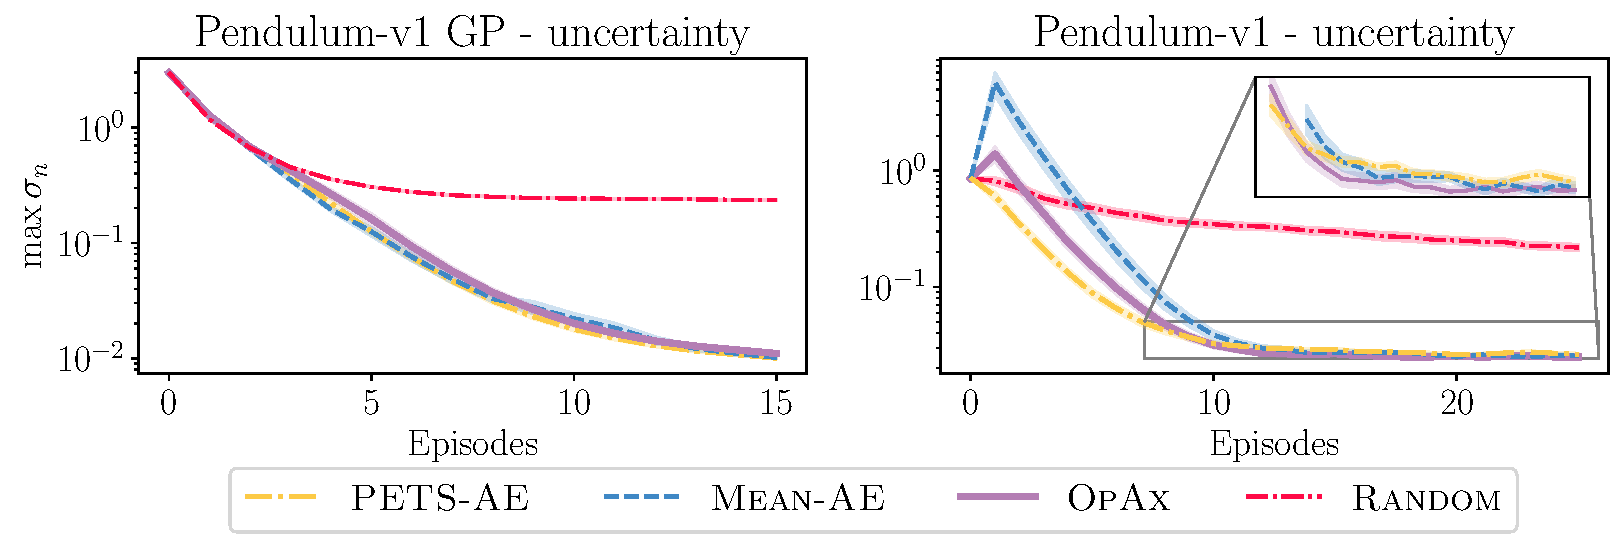
\includegraphics[width=0.9\linewidth]{Latex_Praesentation/figures/uncertainty_plotvalidation_eps_std_max.pdf}
    \vspace{0.05in}

    \begin{center}
        \alert{Active exploration reduces epistemic uncertainty faster than random exploration}
    \end{center}
    
\end{frame}

\begin{frame}{Experiments: Learning and Zero-Shot Generalization (ok)}

    \begin{columns}[T] % Align tops
         \begin{column}{0.4\textwidth}
             \begin{itemize}
                 \item compared to other active exploration baselines, \texttt{OpAx} constantly performs well and is \alert{on par} with \texttt{H-UCRL}
                 \item on the \alert{unseen} tasks the active exploration baselines and \texttt{OpAx} \alert{outperform \texttt{H-UCRL}} by a large margin
             \end{itemize}
         \end{column}
         \begin{column}{0.6\textwidth}
              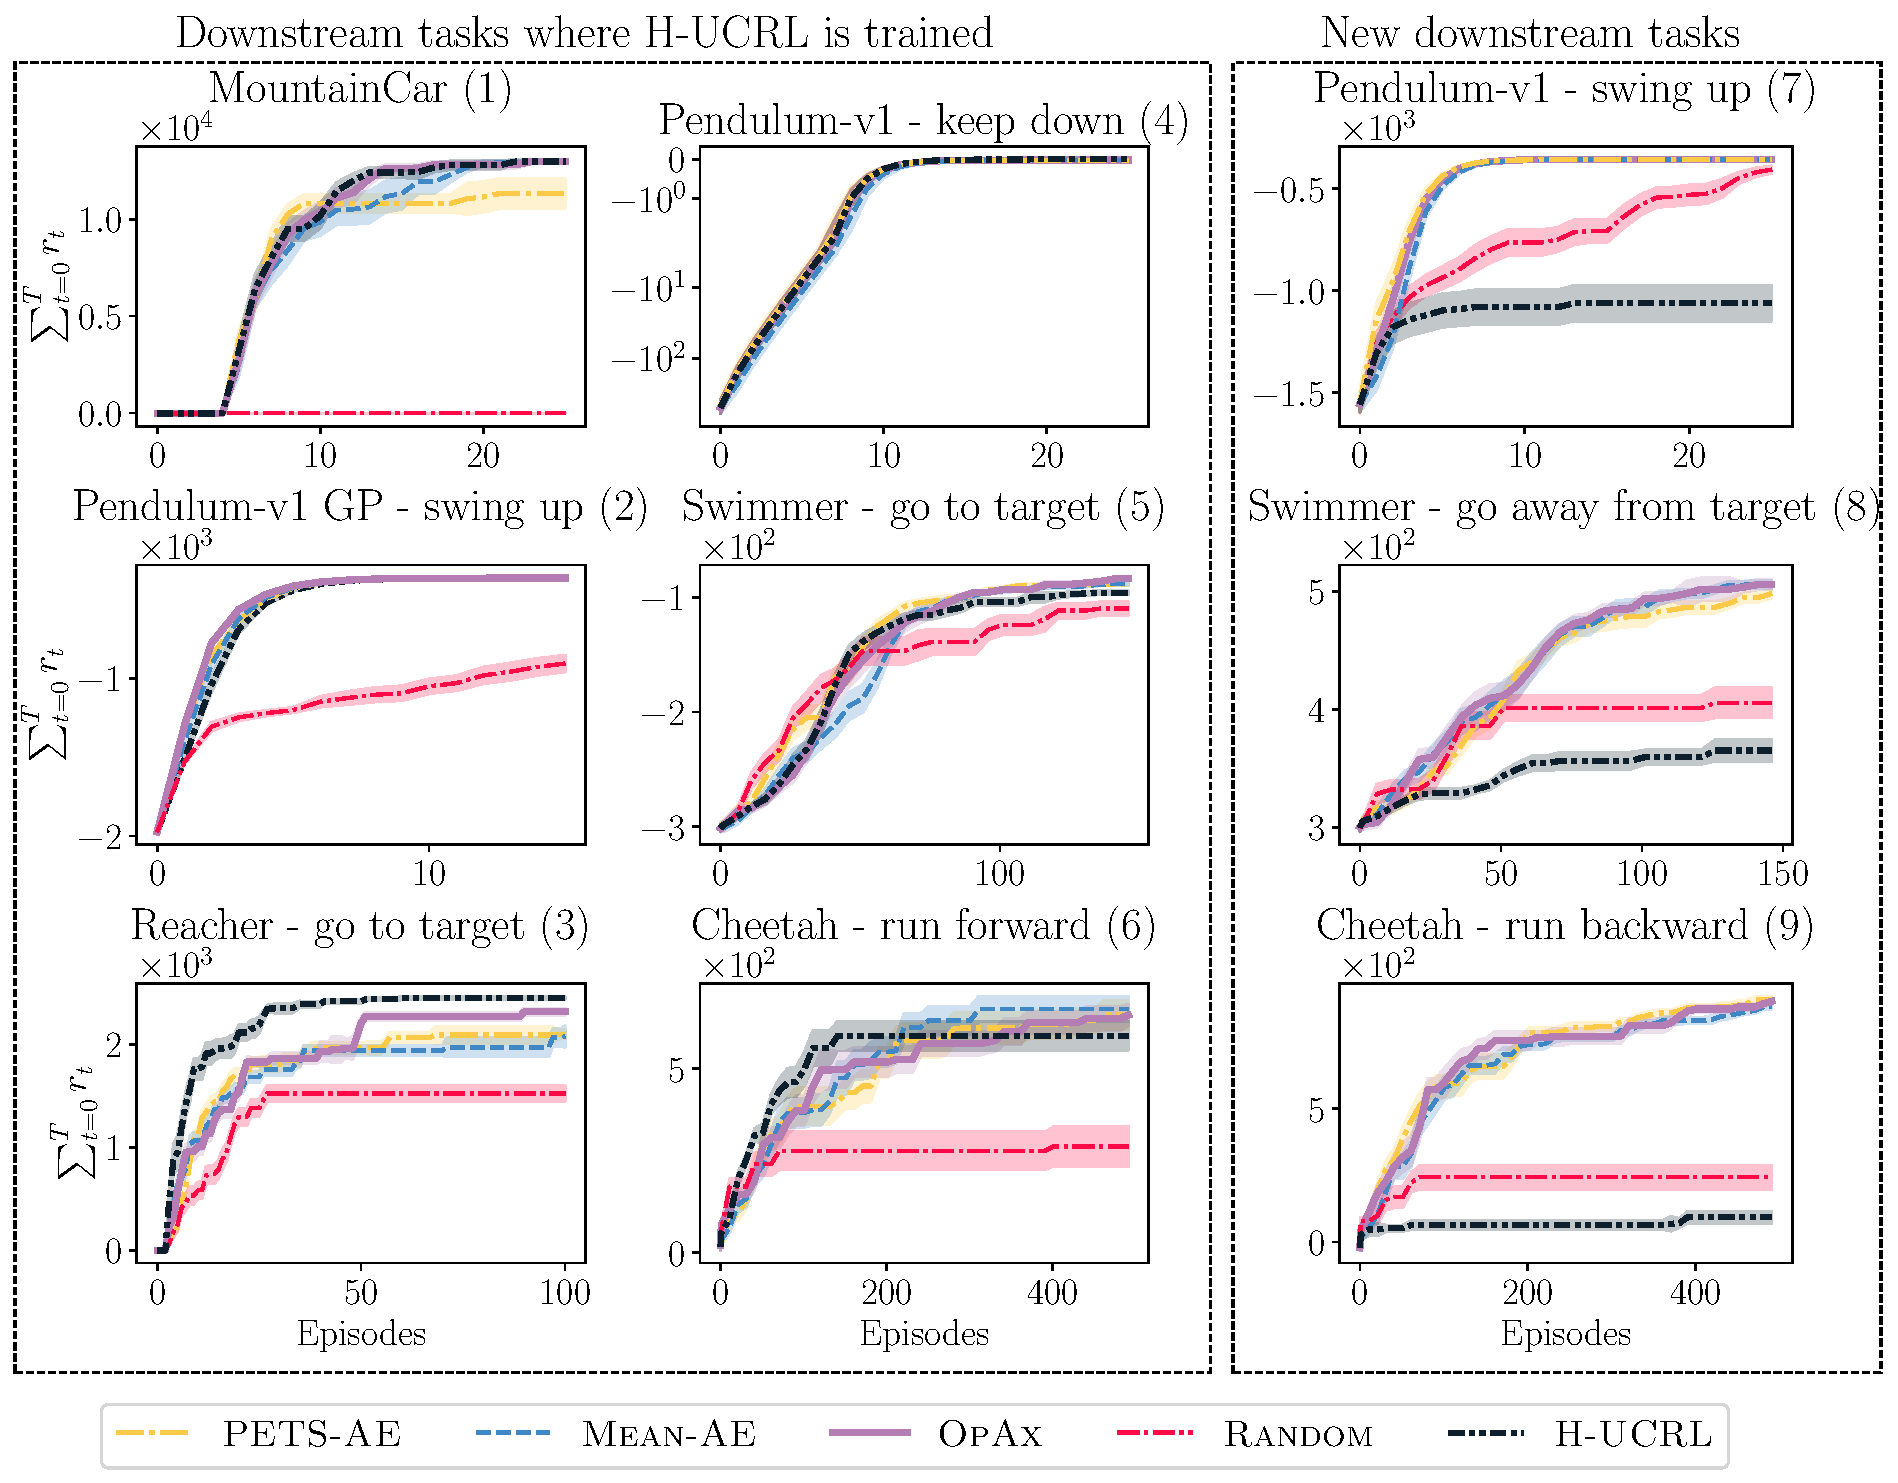
\includegraphics[width=0.99\linewidth]{Latex_Praesentation/figures/results_plot_with_hucrlreward_task_1.pdf}
         \end{column}
     \end{columns}
     
\end{frame}

\begin{frame}{Experiments: Zero-Shot Pendulum Swing-Up (ok)}

    \begin{columns}[T] % Align tops
         \begin{column}{0.5\textwidth}
            \begin{center}
                \movie[label=false,height=0.5\linewidth,width=0.5\linewidth]{\texttt{H-UCRL}}{Latex_Praesentation/videos/hucrl-zero-shot-swingup-4.mov}
            \end{center}
         \end{column}
         \begin{column}{0.5\textwidth}
            \begin{center}
                \movie[label=false,height=0.5\linewidth,width=0.5\linewidth]
                {\texttt{OpAx}}{Latex_Praesentation/videos/opax-zero-shot-swingup-4.mov}
            \end{center}
         \end{column}
     \end{columns}
    \vspace{0.2in}

     \begin{center}
         \alert{Grand statement about \texttt{OpAx}}
     \end{center}
     
\end{frame}

\begin{frame}{Key Findings}
    \begin{itemize}
        \item \textbf{Sample Efficiency:}
        \begin{itemize}
            \item OPAX often reaches target performance with fewer environment interactions.
        \end{itemize}
        \pause
        \item \textbf{Scalability:}
        \begin{itemize}
            \item Successful application to high-dimensional Fetch task using PEs and MPC.
        \end{itemize}
        \pause
        \item \textbf{Objective Robustness:}
        \begin{itemize}
            \item Log-uncertainty objective (Eq. 6) performs similarly to simpler sum-of-uncertainties (OPAX-SUM, Fig 5). Core benefit seems to be optimistic planning towards uncertainty.
        \end{itemize}
    \end{itemize}
\end{frame}

% --- Section 6: Discussion & Conclusion ---
\section{Discussion \& Conclusion}

\begin{frame}{Strengths and Strategic Relevance}
    \begin{itemize}
        \item \textbf{Principled:} Grounded in information theory (Bayesian optimal experimental design).
        \item \textbf{Generalization Focus:} Directly tackles task-specific bias, aiming for versatile world models.
        \item \textbf{Theoretical Support:} Convergence guarantees (esp. for GPs) provide confidence.
        \item \textbf{Novel Optimism:} Applies optimism principle effectively to information gain.
        \item \textbf{Empirically Validated:} Strong performance across diverse benchmarks.
        \pause
        \item \textbf{Strategic Importance:} Contributes to foundational challenge of building agents that autonomously acquire comprehensive world models – crucial for AGI goals (planning, reasoning, adaptation). OPAX offers a concrete algorithm for the data acquisition phase.
    \end{itemize}
\end{frame}

\begin{frame}{Limitations and Open Questions}
    \begin{itemize}
        \item \textbf{Computational Cost:} Optimistic planning (solving Eq. 7) can be expensive, especially for high dimensions / long horizons. Scalability remains a challenge.
        \pause
        \item \textbf{Uncertainty Calibration:} Performance heavily relies on accurate, well-calibrated uncertainty estimates from the probabilistic model. What if uncertainty is poor? (Robustness needed).
        \pause
        \item \textbf{Assumptions:}
        \begin{itemize}
            \item Fully Observed Systems (MDPs): How to extend to POMDPs?
            \item Static Dynamics: How to handle non-stationarity?
            \item Horizon Dependence: Theoretical bounds can depend on $T$.
        \end{itemize}
        \pause
        \item \textbf{Exploration vs. Exploitation:} OPAX is pure exploration. How to best integrate with downstream task execution?
    \end{itemize}
\end{frame}

\begin{frame}{Future Directions}
    \begin{itemize}
        \item \textbf{Scalability \& Efficiency:} Faster optimistic planning approximations (e.g., amortized planning).
        \item \textbf{Robustness:} Design methods less sensitive to uncertainty miscalibration.
        \item \textbf{POMDP Extension:} Information gain in belief space.
        \item \textbf{Advanced Models:} Apply to hierarchical / latent variable models.
        \item \textbf{Lifelong Learning:} Integrate OPAX into agents that learn continuously.
        \item \textbf{Balancing Objectives:} Combine information gain with task rewards during exploration.
        \item \textbf{Real-World Robotics:} Address safety, sample efficiency, physical interaction challenges.
    \end{itemize}
\end{frame}

\begin{frame}{Conclusion}
    \begin{itemize}
        \item OPAX \footcite{sukhija2023optimistic} presents a principled and effective algorithm for \textbf{task-agnostic active exploration} in dynamical systems.
        \pause
        \item By maximizing \textbf{information gain} via \textbf{optimistic planning}, it learns globally accurate models that enable strong \textbf{zero-shot generalization}.
        \pause
        \item Supported by \textbf{theoretical guarantees} and validated by \textbf{empirical results} across diverse environments.
        \pause
        \item Represents a significant step towards building more \textbf{general, adaptable, and data-efficient} learning agents.
        \pause
        \item Key challenges remain in \textbf{scalability} and \textbf{robustness}, offering exciting avenues for future research.
    \end{itemize}
\end{frame}

% --- Bibliography ---
\begin{frame}[allowframebreaks]{References} % allowframebreaks allows bibliography to span multiple slides if needed
    \printbibliography
\end{frame}

% --- Closing Slide ---
\begin{closingframe}

    \begin{center}
        \begin{minipage}{1\textwidth}
            \textbf{Chung-En Tsai}\hfill
            \textit{\email{chtsai@ethz.ch}}
            
            \vspace{0.25em}
            
            \textbf{Ben Bullinger}\hfill\textit{\email{bben@ethz.ch}}
        \end{minipage}
    \end{center}

    \vfill

    \begin{columns}
		\begin{column}{\textwidth}
            ETH Zurich\\
            Department of Computer Science
		\end{column}
	\end{columns}

\end{closingframe}

\end{document}

% --- Dummy references.bib file content ---
/*
@inproceedings{sukhija2023optimistic,
  title={Optimistic Active Exploration of Dynamical Systems},
  author={Sukhija, Bhavya and Treven, Lenart and Sancaktar, Cansu and Blaes, Sebastian and Coros, Stelian and Krause, Andreas},
  booktitle={Advances in Neural Information Processing Systems},
  volume={36},
  pages={45869--45883},
  year={2023},
  url={https://proceedings.neurips.cc/paper_files/paper/2023/file/a4a4cdab45ef4883ed66e49785819a94-Paper-Conference.pdf}
}

% Add other citations from the report if needed, e.g.:
@inproceedings{chua2018deep,
  title={Deep reinforcement learning in a handful of trials using probabilistic dynamics models},
  author={Chua, Kurtland and Calandra, Roberto and McAllister, Rowan and Levine, Sergey},
  booktitle={Advances in neural information processing systems},
  volume={31},
  year={2018}
}

@article{kakade2020information,
  title={Information theoretic regret bounds for reinforcement learning},
  author={Kakade, Sham M and Dann, Christoph and Krishnamurthy, Akshay},
  journal={arXiv preprint arXiv:2006.05211},
  year={2020}
}

@inproceedings{lakshminarayanan2017simple,
  title={Simple and scalable predictive uncertainty estimation using deep ensembles},
  author={Lakshminarayanan, Balaji and Pritzel, Alexander and Blundell, Charles},
  booktitle={Advances in neural information processing systems},
  volume={30},
  year={2017}
}

@inproceedings{haarnoja2018soft,
  title={Soft actor-critic: Off-policy maximum entropy deep reinforcement learning with a stochastic actor},
  author={Haarnoja, Tuomas and Zhou, Aurick and Abbeel, Pieter and Levine, Sergey},
  booktitle={International conference on machine learning},
  pages={1861--1870},
  year={2018},
  organization={PMLR}
}

@inproceedings{curi2020hucrl,
    title =        {{H-UCRL}: Hybrid Uncertainty Estimation for Model-Based {RL}},
    author =       {Curi, Sebastian and Berkenkamp, Felix and Krause, Andreas},
    booktitle =    {Proceedings of the 37th International Conference on Machine Learning},
    pages =        {2224--2233},
    year =         {2020},
    volume =       {119},
    series =       {Proceedings of Machine Learning Research},
    month =        {13--18 Jul},
    publisher =    {PMLR},
}

@inproceedings{li2020generalized,
  title={Generalized Hindsight for Long-Horizon Visuomotor Reinforcement Learning},
  author={Li, Alexander and Pong, Vitchyr H and Florence, Phillip and Agrawal, Pulkit and Levine, Sergey},
  booktitle={Robotics: Science and Systems (RSS)},
  year={2020}
}

@article{chaloner1995bayesian,
  title={Bayesian experimental design: A review},
  author={Chaloner, Kathryn and Verdinelli, Isabella},
  journal={Statistical Science},
  pages={273--304},
  year={1995},
  publisher={JSTOR}
}

@inproceedings{wagenmaker2023certainty,
  title={Certainty-equivalent exploration in latent dynamics models},
  author={Wagenmaker, Andrew J and Ma, Yifan and Boots, Byron},
  booktitle={Conference on Robot Learning},
  pages={1403--1413},
  year={2023},
  organization={PMLR}
}

*/
